\documentclass[11pt]{article}

\usepackage[margin=1.1in]{geometry}
\usepackage{amsmath,amssymb}
\usepackage{booktabs}
\usepackage{graphicx}
\usepackage{url}
\usepackage[colorlinks=true,linkcolor=blue,citecolor=blue]{hyperref}

\newcommand{\norm}[1]{\left\lVert #1 \right\rVert}
\newcommand{\xbar}{\bar{x}}
\newcommand{\R}{\mathbb{R}}

\title{Large $\rho$ does not make progressive hedging diverge on the
farmer problem; it makes the convergence metric lie}
\author{David L.\ Woodruff}
\date{\today}

\begin{document}
\maketitle

\begin{abstract}
Progressive hedging (PH) is usually reported as converged when the primal
residual $\norm{x_s - \xbar}_1$ falls below a threshold.  We ask whether a very
large penalty parameter $\rho$ makes that metric increase --- whether PH
diverges --- on the three-crop, three-scenario farmer problem.  It does not.
For $\rho \ge 10^4$ the metric reaches solver tolerance at the second iteration
and never rises again, while $\xbar$ sits $58$ acres from the extensive-form
solution and creeps toward it at a rate of exactly $172.6/\rho$ acres per
iteration.  We explain the freeze: when $\xbar$ is feasible for the first-stage
constraints, a dominant proximal term makes every subproblem return $\xbar$
itself, and the PH iteration degenerates into a projected gradient step of
length $1/\rho$ on the extensive-form objective.  The metric does increase, by
as much as a factor of $5.4 \times 10^6$ in a single iteration, but at the
intermediate values $\rho \in \{100, 1000\}$ rather than at the large ones.  On
this problem the primal residual measures agreement among subproblems, not
proximity to a solution, and the two are easy to tell apart only if one is
willing to solve the extensive form.
\end{abstract}

\section{Question and setup}

Let $S$ index scenarios with probabilities $p_s$, let $x_s \in \R^n$ be the
first-stage variables of scenario $s$, and let
$\xbar = \sum_s p_s x_s$.  mpi-sppy's \texttt{phbase.convergence\_diff} reports
\begin{equation}
  \label{eq:conv}
  \mathrm{conv} \;=\; \frac{1}{|S|}\sum_{s\in S} \frac{1}{n}\norm{x_s - \xbar}_1 ,
\end{equation}
and terminates PH when this falls below \texttt{convthresh}.  The question is
whether \eqref{eq:conv} increases when $\rho$ is made very large.

We use the farmer problem \cite{birge} in the form distributed with mpi-sppy,
\texttt{examples/farmer/farmer.py}, with \texttt{crops\_multiplier}$\,=1$
(three crops: wheat, corn, sugar beets) and three scenarios (below-average,
average and above-average yields), continuous first-stage acreage variables
$x \in \R^3_+$ subject to the single constraint $\sum_j x_j \le 500$.  The
extensive form solves to
\[
  x^\star = (\text{corn } 80,\; \text{sugar beets } 250,\; \text{wheat } 170),
  \qquad z^\star = -108390 .
\]

Runs use the PH hub alone --- no spokes, no bound-producing cylinders, one MPI
rank --- so that nothing outside the PH iteration can influence the
trajectory.  Each run is $100$ iterations at a fixed $\rho$ with
\texttt{convthresh} set to $-1$ so that no run stops early, solved with Gurobi
through \texttt{gurobi\_direct}.  The metric \eqref{eq:conv} is recorded by a PH
extension whose \texttt{miditer()} callback fires immediately after
\texttt{phbase} assigns \texttt{self.conv}, so the recorded sequence is exactly
the one \texttt{phbase} would have compared against the threshold.

\section{Results}

Table~\ref{tab:sweep} sweeps $\rho$ over nine values spanning nine orders of
magnitude.

\begin{table}[t]
\centering
\begin{tabular}{rrrrrr}
\toprule
$\rho$ & conv$_{100}$ & rises & max jump & $\norm{\xbar - x^\star}_\infty$ & drift \\
\midrule
$0.1$    & $1.0\times10^{-1}$  & 38 & $4.8$               & $0.381$   & $5.2\times10^{-1}$ \\
$1$      & $2.6\times10^{-4}$  & 38 & $4.0\times10^{1}$   & $0.00097$ & $7.0\times10^{-4}$ \\
$10$     & $3.7\times10^{-3}$  & 35 & $3.9\times10^{5}$   & $0.0139$  & $7.9\times10^{-3}$ \\
$10^{2}$ & $8.1\times10^{-9}$  & 46 & $5.4\times10^{6}$   & $32.0$    & $1.3\times10^{-1}$ \\
$10^{3}$ & $9.5\times10^{-8}$  & 39 & $3.5\times10^{5}$   & $47.7$    & $4.3\times10^{-2}$ \\
$10^{4}$ & $8.4\times10^{-8}$  &  2 & $1.2$               & $56.6$    & $1.7\times10^{-2}$ \\
$10^{5}$ & $2.1\times10^{-8}$  &  0 & $1$                 & $58.2$    & $1.7\times10^{-3}$ \\
$10^{6}$ & $1.5\times10^{-8}$  &  0 & $1$                 & $58.3$    & $1.7\times10^{-4}$ \\
$10^{8}$ & $5.6\times10^{-12}$ &  0 & $1$                 & $58.3$    & $1.7\times10^{-6}$ \\
\bottomrule
\end{tabular}
\caption{PH on the three-crop farmer, $100$ iterations, threshold disabled.
``conv$_{100}$'' is \eqref{eq:conv} at the last iteration; ``rises'' counts
iterations after the first at which it increased; ``max jump'' is the largest
single-iteration increase as a ratio; the fifth column is the true distance
from the final $\xbar$ to the extensive-form solution; ``drift'' is how far
$\xbar$ still moved on the last iteration.}
\label{tab:sweep}
\end{table}

Three things are visible.

\paragraph{At large $\rho$ the metric does not rise at all.}  For
$\rho \ge 10^5$ the ``rises'' column is zero: \eqref{eq:conv} is monotonically
non-increasing over the entire run.  It reaches $10^{-8}$ --- Gurobi's
feasibility tolerance, not a meaningful number --- at iteration $2$ and stays
there.  Any threshold a user would plausibly set is met almost immediately.

\paragraph{The reported convergence is spurious.}  At $\rho = 10^5$ the metric
reads $2\times10^{-8}$ while $\xbar$ is $58$ acres per crop away from
$x^\star$; the run has planted $308$ acres of sugar beets where the answer is
$250$.  The fifth column is monotone in $\rho$ over the whole sweep and
saturates at $58.3$, which is the distance from $x^\star$ to the mean of the
three scenarios' individual wait-and-see solutions.  In other words, at large
$\rho$ PH never leaves its starting point.

\paragraph{The metric rises in the middle of the range.}  At $\rho = 100$ and
$\rho = 1000$ it repeatedly falls to $10^{-10}$ and jumps back to order one:
the largest single-iteration increase is a factor of $5.4\times10^6$ at
$\rho = 100$.  These are the spikes in the left panel of
Figure~\ref{fig:traces}.  Each spike is $\xbar$ drifting far enough that one
scenario's linear program flips to a different vertex; the three scenarios
disagree for a few iterations, and the proximal term then pins them back
together.  The run is nonetheless making progress --- the right panel shows the
true error falling throughout --- so the non-monotonicity of \eqref{eq:conv} is
not divergence either.

\begin{figure}[t]
\centering
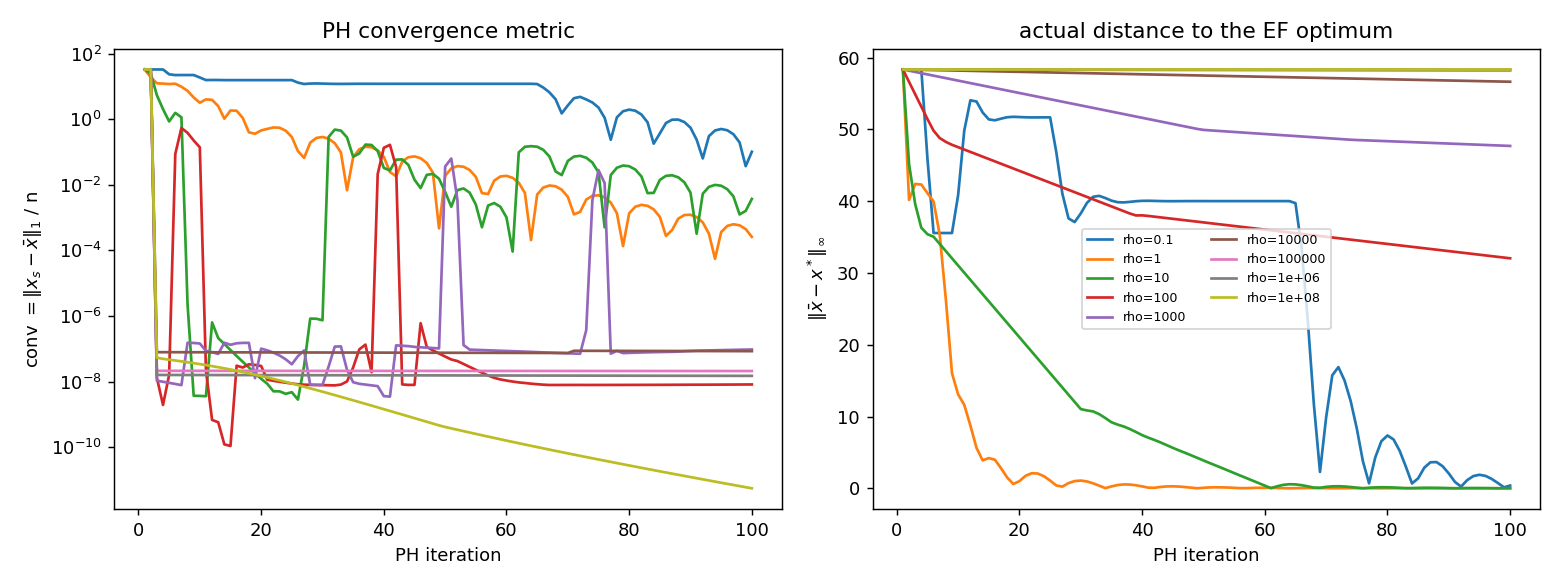
\includegraphics[width=\textwidth]{../farmer_divergence.png}
\caption{Left: the convergence metric \eqref{eq:conv} against iteration, log
scale.  Right: $\norm{\xbar - x^\star}_\infty$ against iteration, linear scale.
The curves that flatten near the top of the right panel are the large-$\rho$
runs whose metric, on the left, has already reached $10^{-8}$.}
\label{fig:traces}
\end{figure}

\section{Why it freezes}

Write the PH subproblem for scenario $s$ at iteration $k$ as
\begin{equation}
  \label{eq:sub}
  x_s^{k+1} \;\in\; \arg\min_{x \in X}\;
    c^\top x + Q_s(x) + (w_s^k)^\top x + \tfrac{\rho}{2}\norm{x - \xbar^k}_2^2 ,
\end{equation}
where $X = \{x \ge 0 : \sum_j x_j \le 500\}$ is the first-stage feasible set and
$Q_s$ is the scenario recourse function.  The essential structural fact about
farmer is that $\xbar^k \in X$ for every $k$: $X$ is convex and $\xbar^k$ is a
convex combination of points of $X$.  As $\rho \to \infty$ the quadratic term
dominates, and the minimizer of \eqref{eq:sub} approaches the projection of
$\xbar^k$ onto $X$ --- which is $\xbar^k$ itself.  Every scenario returns the
same point, the residual \eqref{eq:conv} is zero up to solver tolerance, and PH
declares victory.

The motion that remains is a first-order correction.  Expanding the optimality
condition of \eqref{eq:sub} about $\xbar^k$,
\begin{equation}
  \label{eq:step}
  x_s^{k+1} \;\approx\; \Pi_X\!\left(\xbar^k - \tfrac{1}{\rho}\left(c + w_s^k + g_s^k\right)\right),
  \qquad g_s^k \in \partial Q_s(\xbar^k),
\end{equation}
and averaging over scenarios, using the PH invariant $\sum_s p_s w_s^k = 0$,
\begin{equation}
  \label{eq:pg}
  \xbar^{k+1} \;\approx\; \Pi_X\!\left(\xbar^k - \tfrac{1}{\rho}\left(c + \textstyle\sum_s p_s g_s^k\right)\right).
\end{equation}
The bracket is a subgradient of the extensive-form objective at $\xbar^k$.  So
at large $\rho$, PH is not diverging and is not stalling in any exotic sense:
it has degenerated into projected subgradient descent on the extensive form
with a fixed step length $1/\rho$.  The dual variables $w_s$ have stopped doing
anything, because they only grow through $\rho(x_s - \xbar)$ and $x_s - \xbar$
has been driven to zero.

Equation~\eqref{eq:pg} predicts that the per-iteration motion of $\xbar$ should
scale exactly as $1/\rho$, and it does.  The measured drift multiplied by
$\rho$ is
\[
  172.556,\quad 172.556,\quad 172.555,\quad 172.6
\]
at $\rho = 10^4, 10^5, 10^6, 10^8$ --- constant to five figures over four
decades.  Since the gap to close is $58.3$ acres, reaching $x^\star$ requires
about $58.3\,\rho / 172.6 \approx 0.34\,\rho$ iterations: roughly $34{,}000$ at
$\rho = 10^5$ and $3.4\times10^7$ at $\rho = 10^8$.  The algorithm is correct
and hopeless at the same time.

\section{Discussion}

The practical reading is that on this problem \eqref{eq:conv} is a measure of
agreement among subproblems and not a measure of optimality, and that large
$\rho$ decouples the two completely.  This is worse than divergence would be.  A
diverging metric is visible; a metric that reads $10^{-8}$ while the iterate is
$58$ acres from the answer is not, and it will silently satisfy any termination
test built on it alone.

Two caveats bound the claim.  First, the freeze depends on $\xbar^k \in X$,
which holds here because the first stage has a single knapsack-like constraint
and no integrality.  With integer first-stage variables $\xbar$ is generally
infeasible for the subproblems and the mechanism of \eqref{eq:pg} does not
apply unchanged; whether the metric then rises is a separate experiment.
Second, the sweep is one instance at one scenario count, and the intermediate
$\rho$ behavior in particular --- where the vertex flips live --- should be
expected to depend on the geometry of the recourse function.

The obvious defense is to not rely on the primal residual alone.  A dual
residual, $\rho\norm{\xbar^{k+1} - \xbar^k}$, is exactly the quantity
\eqref{eq:pg} says is constant at $172.6$ here, and would have flagged all four
large-$\rho$ runs as unconverged.  That this is available essentially for free
suggests it belongs in the default termination test rather than beside it.

\section{Reproducing}

Everything is in \texttt{examples/farmer/divergence} on the
\texttt{divergence\_study} branch:

\begin{center}
\begin{tabular}{ll}
\toprule
\texttt{farmer\_ph\_divergence.py} & driver; sweeps $\rho$, writes the table, csv and figure \\
\texttt{farmer\_divergence.csv}    & per-iteration $\rho$, conv, $\norm{w}_\infty$, error, $\xbar$ \\
\texttt{farmer\_divergence.png}    & Figure~\ref{fig:traces} \\
\texttt{notes.md}                  & the same findings in brief \\
\bottomrule
\end{tabular}
\end{center}

\noindent
\texttt{python farmer\_ph\_divergence.py --itermax 100} reproduces
Table~\ref{tab:sweep}.

\begin{thebibliography}{9}
\bibitem{birge} J.\ R.\ Birge and F.\ Louveaux,
  \emph{Introduction to Stochastic Programming}, 2nd ed., Springer, 2011.
\bibitem{rw} R.\ T.\ Rockafellar and R.\ J.-B.\ Wets,
  Scenarios and policy aggregation in optimization under uncertainty,
  \emph{Mathematics of Operations Research} 16(1):119--147, 1991.
\end{thebibliography}

\end{document}
